\documentclass[tikz,border=10pt]{standalone}
\usepackage{tkz-euclide} % 用于绘制直角符号更方便

\begin{document}
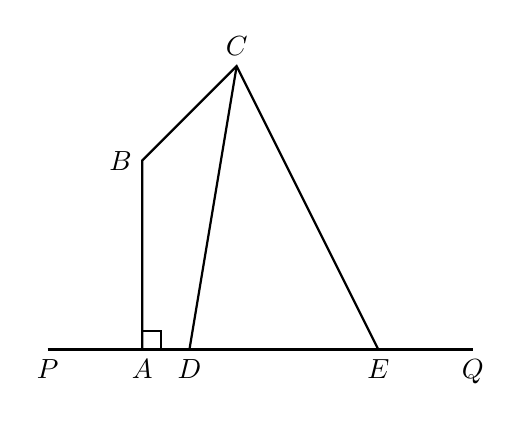
\begin{tikzpicture}[scale=1.2, thick, >=stealth]
    % 1. 定义关键点坐标
    \coordinate (P) at (-1, 0);
    \coordinate (A) at (0, 0);
    \coordinate (D) at (0.5, 0);
    \coordinate (E) at (2.5, 0);
    \coordinate (Q) at (3.5, 0);
    
    \coordinate (B) at (0, 2);      % B在A正上方
    \coordinate (C) at (1, 3);      % C是顶点
    
    % 2. 绘制主要直线和线段
    \draw (P) -- (Q);               % 绘制直线 PQ
    \draw (A) -- (B) -- (C) -- (E); % 绘制外轮廓折线
    \draw (C) -- (D);               % 绘制线段 CD
    
    % 3. 绘制直角符号 (在点A处)
    \draw (0, 0.2) -- (0.2, 0.2) -- (0.2, 0);
    
    % 4. 标注点名称
    % 参数解释: below(下方), left(左侧), above(上方)
    \node[below] at (P) {$P$};
    \node[below] at (A) {$A$};
    \node[below] at (D) {$D$};
    \node[below] at (E) {$E$};
    \node[below] at (Q) {$Q$};
    
    \node[left]  at (B) {$B$};
    \node[above] at (C) {$C$};

    % (可选) 如果需要强调点，可以画出小圆点
    % \foreach \p in {A,B,C,D,E} \fill (\p) circle (1.5pt);

\end{tikzpicture}
\end{document}